% Figure: EMF Compare time per component against component size (MoDisco case study).
% Data: component-compare-summary.md of the eight-component run (168,992 ms total)
% and of the recheck on 2026-03-24 (186,696 ms total). Sizes are XMI bytes / 2^20.
% Colors: categorical slots 1 and 2 of the validated default palette; the marker
% shape differs per series so identity never depends on color alone.
\documentclass[border=2pt]{standalone}
\usepackage{pgfplots}
\pgfplotsset{compat=1.18}

\definecolor{ink}{HTML}{0B0B0B}
\definecolor{inksoft}{HTML}{52514E}
\definecolor{axisgray}{HTML}{C3C2B7}
\definecolor{gridgray}{HTML}{E1E0D9}
\definecolor{seriesone}{HTML}{2A78D6}
\definecolor{seriestwo}{HTML}{EB6834}

\begin{document}
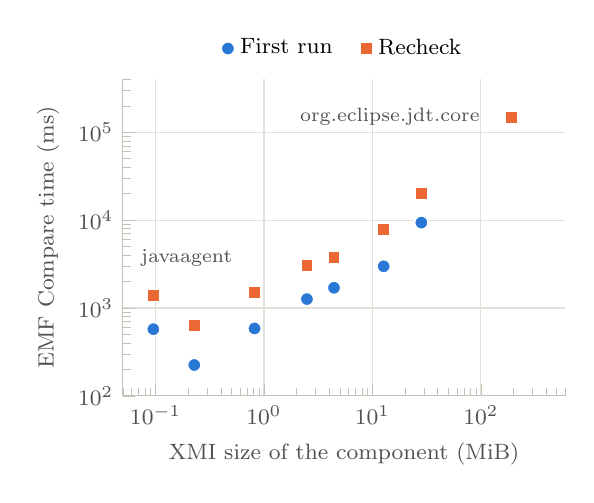
\begin{tikzpicture}
\begin{loglogaxis}[
  width=7.2cm, height=5.6cm,
  font=\footnotesize,
  xmin=0.05, xmax=600, ymin=100, ymax=400000,
  xlabel={XMI size of the component (MiB)}, ylabel={EMF Compare time (ms)},
  axis line style={draw=axisgray}, tick style={draw=axisgray},
  axis x line*=bottom, axis y line*=left,
  grid=major, major grid style={draw=gridgray, line width=0.4pt},
  label style={text=inksoft}, tick label style={text=inksoft},
  legend style={draw=none, fill=none, legend columns=2, at={(0.5,1.03)}, anchor=south,
    /tikz/every even column/.append style={column sep=8pt}},
  legend cell align=left,
]
\addplot[only marks, mark=*, mark size=2.4pt, mark options={fill=seriesone, draw=white, line width=0.5pt}]
  coordinates {
    (0.0955,573) (0.2277,224) (0.8184,584) (2.4909,1261)
    (4.4242,1696) (12.6896,2977) (28.2484,9362) (191.6174,152315)};
\addplot[only marks, mark=square*, mark size=2.2pt, mark options={fill=seriestwo, draw=white, line width=0.5pt}]
  coordinates {
    (0.0955,1385) (0.2277,632) (0.8184,1496) (2.4909,3064)
    (4.4242,3787) (12.6896,7748) (28.2484,20283) (191.6174,148301)};
\legend{First run, Recheck}
\node[font=\scriptsize, text=inksoft, anchor=east] at (axis cs:120,150000) {org.eclipse.jdt.core};
\node[font=\scriptsize, text=inksoft, anchor=south west] at (axis cs:0.06,2300) {javaagent};
\end{loglogaxis}
\end{tikzpicture}
\end{document}
